%%%%%%%%%%%%%%%%%%%%%%%%%%%%%%%%%%%%%%%%%%%%%%%%%%%
%
%  New template code for TAMU Theses and Dissertations starting Fall 2012.  
%  For more info about this template or the 
%  TAMU LaTeX User's Group, see http://www.howdy.me/.
%
%  Author: Wendy Lynn Turner 
%	 Version 1.0 
%  Last updated 8/5/2012
%
%%%%%%%%%%%%%%%%%%%%%%%%%%%%%%%%%%%%%%%%%%%%%%%%%%%

%%%%%%%%%%%%%%%%%%%%%%%%%%%%%%%%%%%%%%%%%%%%%%%%%%%%%%%%%%%%%%%%%%%%%%
%%                           SECTION I
%%%%%%%%%%%%%%%%%%%%%%%%%%%%%%%%%%%%%%%%%%%%%%%%%%%%%%%%%%%%%%%%%%%%%
%\fancypagestyle{alim}{\fancyhf{}\renewcommand{\headrulewidth}{0pt}\fancyfoot[R]{This thesis follows the style for IEEE journal of}}





\pagestyle{myheadings} % No headers, just page numbers
\pagenumbering{arabic} % Arabic numerals
\setcounter{page}{1}

\chapter{\uppercase {Introduction and Background}}
\section{Overview}
%\justify

\setlength{\parindent}{2em}
\indent 
	Predicting or forecasting demand for a product or service is now a common exercise for companies before or after launching a product in order to improve it for the customers. This type of forecasting is possible because of the availability of the ``Big Data". Big Data delivers many potentially breathtaking opportunities for researchers for discovering knowledge which is proving to be very valuable for any companies growth in the market share. However, forecasting using Big Data is not something which is free from challenges. It raises few questions which is also needed to be answered theoretically and methodically. Suppose, the significance of the data that can be found today, might show representation of what’s happening currently (Now casting) or a very good tool to study for predicting what might happen in future (Forecasting). Methodically, there is also a need to prevent picturing unreliable conclusions also most importantly finding ways to reduce the dimensionality of the current Big Data and use it to find important knowledge.   
\blfootnote{This thesis follows the style of the IEEE transaction on Neural Networks and Learning Systems.} 

Accurately demand forecasting paves new ways for improvement in many real world applications~\cite{hart2012demand}. It helps organizations to reduce costs, take smart decisions and increase efficiency. From health care to energy to transportation, demand forecasting is helping researchers or decision makers to make better selections and crack problems which has a long lasting effect. The foundation of this forecasting technique came from the century old disciplines of statistics and mathematics. Continuous improvement of analytics and mathematics lead us to this era of ``Machine learning", which is proving its worth as the data is getting bigger and bigger and going out of reach of human's computational power. 

The intent behind the chosen research topic is to get more deep into these demand forecasting methods and find some reasonable ways to do forecasting. It is impossible to focus into every types of demand forecasting as the numbers of fields related to it is increasing day by day. Therefore, for this thesis transportation demand forecasting was selected and an important section of it (Bike Sharing System) was studied. Bike sharing system is an entertaining, enjoyable and also an affordable way of moving around the town. It is therefore, getting a lot of attention as well as subscribers who uses this transportation medium in a daily basis. Like any other service it is also not free from problems and bike rebalancing is in the top. 

Hence, this thesis focuses on the bike share data and try to forecast rental demand from it to find a way to solve this bike rebalancing problem. The proposed method is a Convolutional Neural Network based~\cite{krizhevsky2012imagenet} forecasting technique to forecast hourly bike rental demand for both genders (male and female). This forecasting is also described as a regression problem with the time series feature and these features were restructured as images in order to be trained on the CNN model. This method is trained and tested on the historical dataset from the City Bike Trip records of New York City. The evaluation results also shows that proposed method is performing better than the conventional machine learning methods.  




\subsection{Demand Forecasting}
\label{DF}


Doing demand forecasting or forecasting in general using Big Data, we can achieve reliable estimation by scrutinizing and finding useful hidden patterns in the data. According to~\cite{richards2013three} data related decision making can improve predictions. Tucker~\cite{tucker} also thinks that Big Data will be able to predict our every move really soon. Therefore, we end up asking ourselves one question- ``what problems are there while tying to forecast with Big Data?" According to~\cite{madden2012databases} the easiest answer is the size, complexity and the speed of data is unmanageable. Also the variations in data and absence of a common structure makes traditional tools and techniques really difficult to use~\cite{arribas2014accidental}. Which is then poses a big problem for the organizations out there who are trying to forecast different types of demands. For example, organizations like European central bank also organized whole workshop only focusing on forecasting using Big Data. 


\section {Methodologies}
\label{methods}

Forecasting is everywhere and for many many years people have been doing a lot of different types of forecasting such as - weather prediction, sports outcomes, political and economical event and so on. As we try to predict a lot of different events, therefore, a lot of different methods can also be applied to do that. Using naive instinct, specialist opinions, or using past events data and match with traditional time series and statistical techniques are just a few.

These demand forecasting are continuously improving with the introduction of latest data mining and machine learning techniques but there is no specific method that allows organizations to foresee future ambiguities and risks. Commonly there are two approaches for forecasting demand - 

\begin{enumerate}
\item Survey Methods
\item Statistical Methods
\end {enumerate}


\subsection {Survey Methods for Demand Forecasting }
\label{survey}

To forecast demand for a short term, survey method is one the most common and straight forward method out there. The goal of this method is to get the intentions of the consumers about their future purchase ideas and help the organizations to create better plans. This is done by conducting surveys with consumers about the current product and determine the demand and services to predict the future demand. This method relies on three different exercises such as - Experts opinion poll, Market experiments and Delphi method (a group decision making technique).  

\subsection{Statistical Methods for Demand Forecasting}
\label{Statsistics}

Statistical methods are complex set of methods which are used to forecast demand in the long run. Demands are mostly forecasted on the availability of the historical and cross sectional data. Unlike the survey methods, statistical methods are reliable and cost effective because of the minimum element of subjectivity. There are a lot of different statistical methods out there like- Trend projection method, Barometric methods and so on. But a very popular and reliable method is to do `Machine Learning' and `Deep Learning' based demand forecasting. A brief details about them is given below. 



\subsubsection{Machine Learning for Demand Forecasting}
\label{MachineLearning}

Nowadays automated detection of meaningful patterns in data is denoted by Machine Learning. The usage of machine learning has grown significantly in the past couple of decades and became a very common tool in order to extract information from a huge sets of data. Machine learning applications are also making our everyday life lot easier, starting from- search engines, which knows how to fetch the best and most relevant results. Anti-virus, spam, fraud software’s- to filter our data, mail, credit card fraud detection, autonomous or collision prevention on cars, as well as in a lot of applications on the fields of medicine, astronomy etc. I this case machine learning methods has been a great success for demand forecasting based on historical data. 

Before going too deep into machine learning we also should know when we need machine learning. We mainly need the shelter of machine learning when a task becomes too complex to program. 
\begin{itemize}
\item These kind of task may be performed by humans or animals such as driving, speech recognition or image processing. Therefore to deal with this kind of problem, machine learning tools comes in handy, as it can learn from past experience or data in order to provide adequate results. 
\item These task can be beyond human capabilities- such as analysis of big complex data sets of astronomic data, predicting or forecasting future, converting medical data into knowledge, recommendation system etc. 
\end{itemize}

There are two different types of machine learning tool - 
\begin{enumerate} 
\item Supervised: When the manually labelled dataset is provided to carryout future work. 
\item Unsupervised: to describe the hidden structure of the unlabeled data. 
\end{enumerate} 
In this thesis, I have dealt with supervised machine learning where I used labelled bike sharing service data to do the forecasting task of the system.


\subsubsection{Deep Learning for Demand Forecasting}
\label{DeepLearning}

Trying to mimic the human brain with the robustness and efficiency and adeptness it exemplifies has always been the main challenge in AI (Artificial intelligence) research field. Humans are capturing countless data every second and still capable of finding the good use of those in future use with a crisp method. And in neuroscience research they are developing new ideas for designing systems which represents various types of information based on the findings that provides insights of the representation of the human brains. This new method leads to the breakthrough of the Deep learning which emphases on the computational models for useful knowledge representation just like the neocortex. In neocortex rather than explicitly processing signals it permits them to proliferate through a very complex order of parts in a way that overtime it will learn to provide observations based on their regularities. Therefore, deep learning can produce a new representation of the data and solve very complex forecasting models like demand forecasting.

In simple words, Deep learning is a complex level of machine learning algorithm where - 

\begin{itemize}
\item It consists of many levels of layers which are used to extract features from the input. Every layer uses its previous layers output as their input. 

\item It can be supervised or unsupervised.

\item It forms a hierarchical representation by originating higher level features from the lower level features. 

\item The composition of these layers are dependent of the problem it is trying to solve. 

\item At each layer, like an artificial neuron the signals are transformed and the parameters of these neurons are learned through the training of the network.

\end{itemize}


Based on the application and framework it is being used every deep learning algorithm has their own strength and weaknesses. In this thesis I have used one of the well established and popular method Convolutional neural network (CNN) to solve the forecasting problem of the bike sharing system. 

\subsubsection{Convolutional Neural Network}
\label{CNN}



To solve the goal of the thesis the method I used is the Convolutional neural network which is a very popular deep learning method. It is a kind of feed forward artificial neural network where the neurons connectivity patterns are enthused from the visual neocortex of the animals \cite{o2015introduction}. This biologically inspired machine learning method is included with some self optimizable neurons through learning. Starting from the input vector to the output result, the whole network states a single weight function by keeping the traditional neural networks regular ideas and adding some special features to it. 

\textbf{Architecture:}
One of the main difference between the artificial neural network and CNN is, CNN consists of neurons of three dimensions [figure~\ref{anncnn}]. These are the spatial dimensionality of the input width and height, and the depth. Also the neurons of a CNN in any specified layer is associated to a minor area of the layer prior to it. 

In overall, CNN is consists of three different types of layer - Convolutional layer, Pooling layer and the Fully connected layer. 




\begin{figure}
\centering
\begin{adjustbox}{addcode={\begin{minipage}{\width}}
{\caption{Architechture of the traditional Artificial Neural Network (ANN) (above) and the Convolutional Neural Network (CNN)  (below). } 
\label{anncnn}
\end{minipage}}}
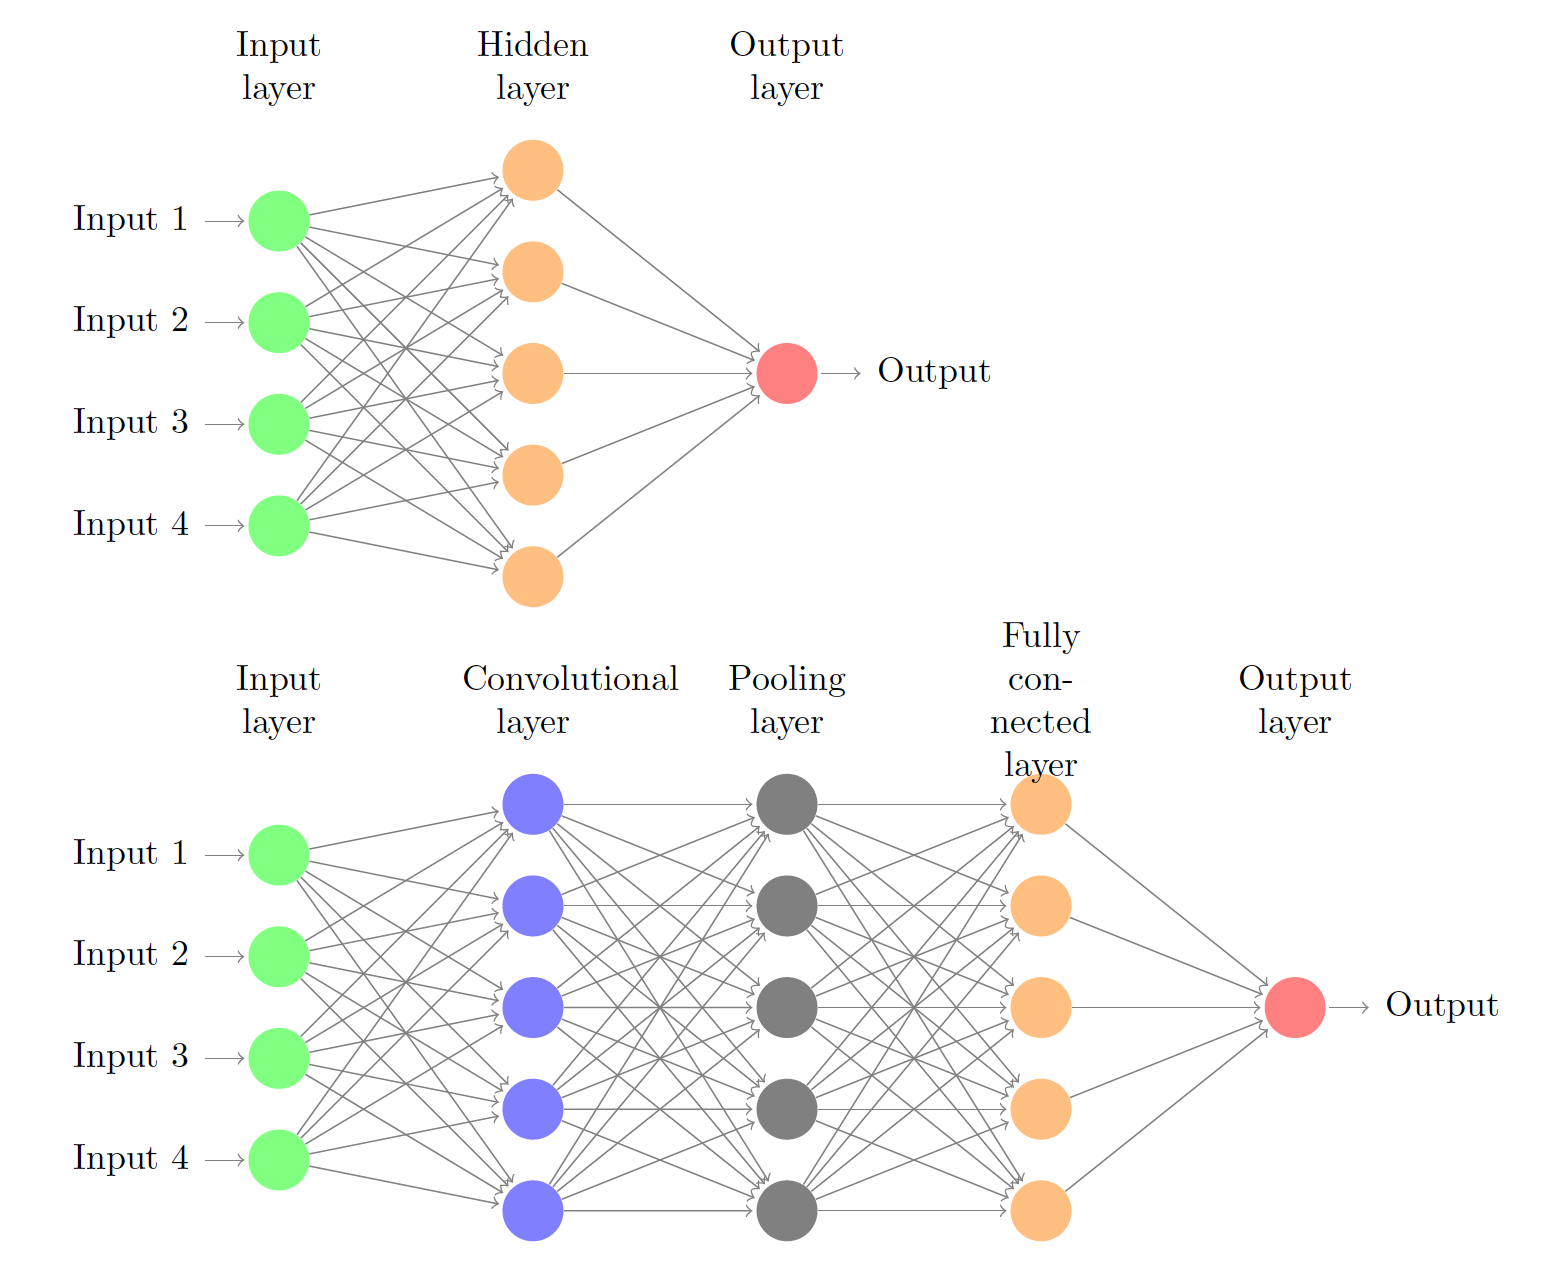
\includegraphics[scale=0.563]{figures/NN_arch.png}
\end{adjustbox}
\end{figure}


The key functionality of the CNN layers can be described in the following areas: 

\begin{itemize}

\item The input layer of CNN will work as same as the ANN input layer by distributing the input values to the next level of layer.
 

\item The next layer of the CNN is the `Convolutional layer'. This layer regulates the output of the neurons connected to the local area of the input. This process is done by the scalar product of the local input area and the weights. Each neuron of this layer takes input from the previous layers rectangular section. Therefore, convolutional layer is an image convolution of the previous layer. 

\item The down-sampling by the spatial dimensionality of the connected input area is then performed by the next layer which is the `Pooling layer'. This layer takes a small block from the convolutional layer and produces a single output by subsampling. Therefore, this layer reduces the number of bounds are placed in that activation. 

\item `Fully connected layer' performs just like it works on a traditional artificial neural network. This layer produces the class scores of the activations. This scores are then used for doing different types of classifications. Also in order to improve overall performance ReLU (rectified linear units) can also be used between these layers. 



\end{itemize}

More mathematical operations about CNN are discussed in the later part of the thesis. 

\begin{figure}
\centering
\begin{adjustbox}{addcode={\begin{minipage}{\width}}
{\caption{A sample Convolutional neural network architecture~\cite{convolutionalneuralnetworks} } 
\label{cnn}
\end{minipage}}}
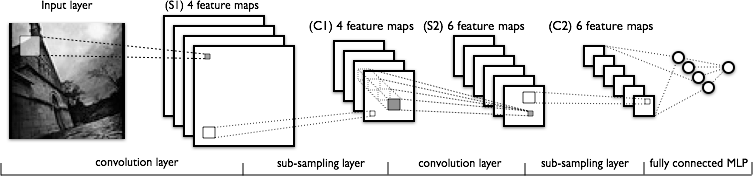
\includegraphics[scale=0.7]{figures/CNNarch.png}
\end{adjustbox}
\end{figure}






\subsection{Big Data \& its Challenges}
\label{int:Challenges} 
In order to state a huge amount of data which can not be handled by the traditional data management methods because of the size and the complexity of the data, the term ``Big Data" was first introduced by Roger Magoulas from O’Reilly media in 2005. According to Sam Madden an associate professor of MIT, Big Data is ``data that's too big, too fast, or too hard for existing tools to process."  

%[[[[ADD big data DEFINIIONS FROM Forecasting with Big Data: A Review]]]]


To overcome this Big Data and extracting information from it we should discuss the 5 V's of the Big Data. These 5 V's includes describing the size of the data (Volume) of different categories (Variety) below the manageable rate (Velocity) and the authenticity (Veracity) as well as the importance of the data(Value) [figure~\ref{5v}].



\begin{figure}
\centering
\begin{adjustbox}{addcode={\begin{minipage}{\width}}
{\caption{5 V's of Big Data } 
\label{5v}
\end{minipage}}}
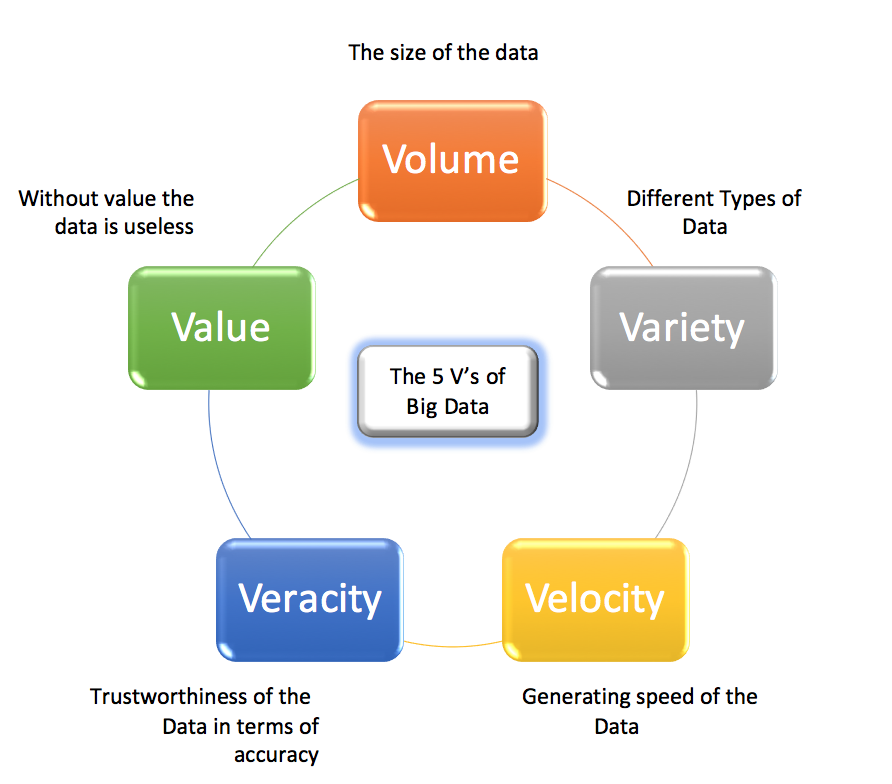
\includegraphics[scale=0.7]{figures/5_vs_safat.png}
\end{adjustbox}
\end{figure}

In order to forecast future,  some important challenges often develops from the nature of the data. Few of them are listed below.


\begin{enumerate} 
\item Statistical impact:  Without getting mislead by randomness, it is important to get precise and significant statistical results. 
\item Analytics construction: There is no fixed rule or way to decide the optimal architecture of the analytic system. 
\item Disseminated mining: To have distributed versions of the methods used, it is must to carryout a lot of research work and theoretical and practical analysis. 
\item Data compression: Storing big data efficiently is also a very important challenge when it comes to Big Data. We can either store the important parts of the data or we can sample the data in a way where we think data is more relevant.
\item Time changing data: Sometimes data changes a lot over the time, for this thesis the data changes significantly over the time. Therefore, it is important for used methods to adapt over the time.
\item Visualization: Another important challenge with dealing with big data is to analyze how to visualize the data to find/solve the problem. 
\end{enumerate}

By overcoming these challenges my goal was to forecast the bike share usage of New York City as well as to find different ways to improve this bike share service. In my thesis, I have considered a set of bike share usage data as image processing problem and in the following part of my thesis I will discuss more about my method and why I chose this approach.



\section{Thesis Outline}
\label{outline}

This thesis is structured in the following sections :

Chapter 2, begins with a review of demand forecasting with Big Data and the problems and potentials are presented, as well as some challenges and applications. This chapter also provides some reviews on the approached topic of bike share service demand forecasting.  
Chapter 3, explains the problem of bike share service and then presents the details about the dataset which was used to build the forecasting model. Furthermore, a few preliminary analysis of the data as well as the methodology of the proposed model is described.    
Chapter 4, presents the feature selection process of the data and brief explanations of the baseline models and evaluation metrics followed by the results and discussions of the proposed model. 
Chapter 5, summarizes the contribution of the thesis as well as some future works are mentioned. 







